\chapter{Introduction} \label{chap1}
	\section{Background}
		Multicarrier Modulation (MCM) is a widely used technique in  broadband communication systems. This  technique  divides the transmitted data into several symbol streams of lower data rate and then transmits these substreams adjacently through subchannels  after being modulated by subcarriers. The aim is to have bandwidth of each subchannel below the coherence bandwidth of the total channel, leading to flat fading subchannels \cite{2005-goldsmithBook}.
		\par The most common scheme of MCM is Orthogonal Frequency Division Multiplexing (OFDM).  \citeauthor{1971-weinstein} \citeyear{1971-weinstein}, made a major breakthrough in the implementation of multicarrier modulation. They proposed using Inverse Fourier Transform (IDFT) for modulation and Discrete Fourier Transform (DFT) for demodulation. It may be referred to as FFT-OFDM since the complexity of calculating N-DFT points can be reduced using Fast Fourier Transform (FFT).
		\par Wavelets and filter banks are alternative methods to represent signals. They have been used in many applications like image processing and communication systems since 1980s. Unlike Fourier transform, wavelet transform uses short waves instead of long waves. When transforming to the frequency domain in Fourier transform, time information is lost. Wavelet transform was introduced to overcome this serious drawback of Fourier transform since it becomes possible to know when an event has occurred. Because of this and other properties of wavelet transform, they have been proposed in some literature to replace FFT-OFDM systems~\cite{1996-strang}.
		\par Impulsive Noise (IN), characterized with short durations and very high
		amplitudes, is identified as an impairment that degrades performance of communication systems. It could be generated from  man-made or atmospheric made sources. These may include switching noise, automobile engine noise, interfering electromagnetic pulses, and so on. Buses, circuits that connect the main parts of a computer, and clocks produce significant noise in laptop and desktop computers as well \cite{2011-nassar-mitigating}.
	\section{Problem Statement and Its Significance}
		Various types of noise can severely affect a wide range of communication systems. One of these noise sources is impulsive noise. For example, in a high speed Digital Subscriber Loop (DSL), impulsive noise sources may include lightning surges, vehicle ignitions, engine noise, electromagnetic discharge, transmission and switching gears \cite{2006-zhidkov}. 
		\par One of the studies on the effect of impulsive noise in ADSL found that without mitigating impulsive noise,  impulses on ADSL lines could be  $ 20-40 $ dB larger than either Additive White Gaussian Noise (AWGN) or near-end crosstalk; hence,  a noise margin of 6 or 12 dB is not sufficient to protect ADSL from impulsive noise. Similarly, in Digital Video Broadcasting (DVB) systems, sources of impulsive noise seem to be the same as those of DSL \cite{2011-mawali}.
		\par In Power Line Communication (PLC) systems, impulsive noise is considered the main reason for frames retransmission scenario \cite{2009-Zbydniewski}. Unlike other communication environments, a channel in PLC is very difficult to model~\cite{2011-mawali}. It was found that the power spectral density (PSD) of impulsive noise is $ 50 $ dB higher than background noise \cite{2011-mawali}.
		In conventional OFDM systems (FFT-OFDM), it is required to add extra load, called the Cyclic Prefix (CP), to compensate for a high degree of spectral overlap.  
		\par As stated in one of the IEEE 802.16.3 proposals, overhead in wavelet-OFDM is less than  of the FFT-OFDM because it does not require the addition of cyclic prefix. For wireless transmission, FFT-OFDM has a cyclic prefix of 20\%; hence, wavelet-OFDM has an advantage of about 20\% in bandwidth efficiency. Moreover, there is no need for pilot tones in wavelet-OFDM systems; however, some Fourier-OFDM systems use 4 out of 52 subbands for pilots which provide additional 8\% advantage for wavelet-OFDM over FFT-OFDM implementations. Finally, unlike Fourier transform, wavelet transform can convert an input domain of real numbers to  an output range of real numbers; hence, reducing the complexity of computation. Because wavelet-OFDM has higher spectral containment, i.e., overlapping, between sub-channels than FFT-OFDM, wavelet-OFDM is able to ameliorate the effects of narrowband interference and is more robust with respect to intersymbol interference and intercarrier interference \cite{2004-zhao}.
		While most works  have considered only FFT-OFDM, our work is directed to reduce the problem of impulsive noise in wavelet-OFDM.
	\section {Scope}
	 	This thesis focuses on wavelet-OFDM systems, particularly, the one which is described in \cite{2011-abdullah} with three different wavelet families Haar, Daubechies-4 and biorthogonal-4.4. Majority of related works have considered mitigation of  impulsive noise problem in FFT-OFDM systems. In this thesis, the performance of FFT-OFDM compared with that of wavelet-OFDM in unmitigated impulsive noise environment.
		\par Other aspects and challenges related to OFDM systems in general, like peak to average power ratio (PAPR) and frequency-timing offset are not considered in this work. The performance of a communication system is well- characterized by two curves, namely, spectral efficiency and bit error rate curves. However, this work focuses on performance in terms of bit error rate only.
	\section{Research Objectives}
	 	The following are the objectives of this work:
		\begin{compactenum} [\hspace*{0.65cm}i.\hspace*{.4cm} ]
			\item To evaluate the performance of the system in terms of bit error rate (BER) and signal to noise ratio (SNR).
			\item To compare the system performance using different wavelet families.
			\item To develop a technique capable of mitigating impulsive noise in wavelet-OFDM system.
		\end{compactenum}
	\section{Research Methodology}
		The research starts with a literature review to cover basic concepts of the topic and related works in the area. After gaining enough background of the problem under investigation, a system model to be simulated and analysed. This will be followed by a study of the effect of impulsive noise in both wavelet-OFDM and Fourier transforms based OFDM systems. Benefiting from other works in the area, a technique will be developed to mitigate impulsive noise in wavelet-OFDM systems. The methodology of this research is shown in a flow chart diagram in Figure~\ref{fig1:method}
		\begin{figure}[p]
			\centering
			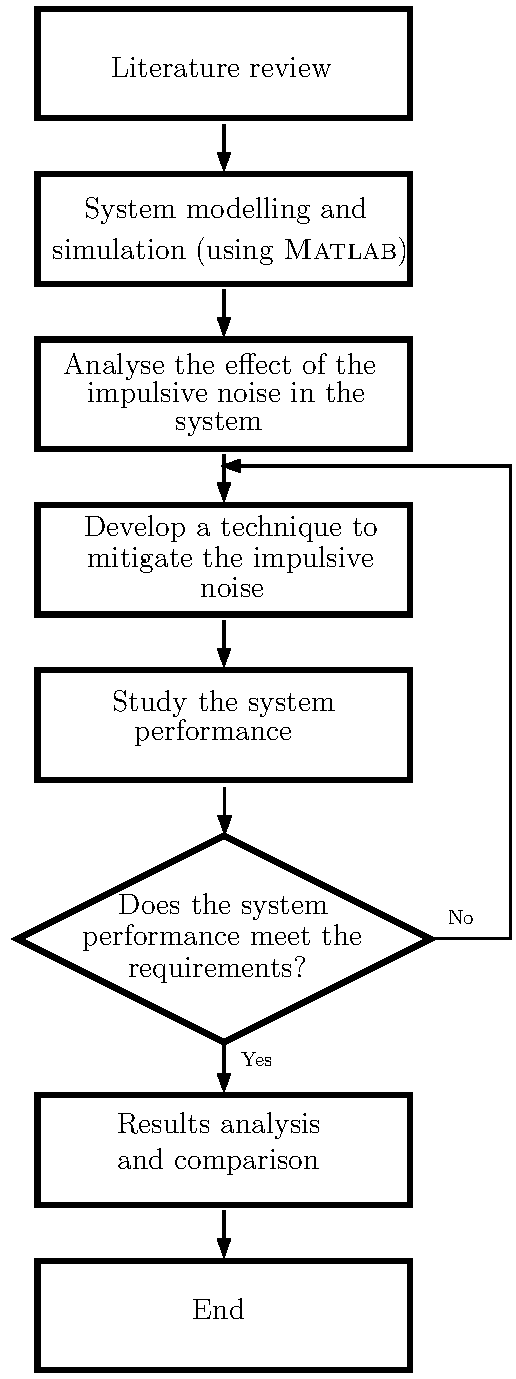
\includegraphics[scale=1]{./chap_1/method}
			\caption{Research methodology.}
			\label{fig1:method}
		\end{figure}
	\section{Thesis Organization}
		This thesis is divided into six chapters. Chapter~\ref{chap1} is the introduction and contains background, problem statement, research methodology and the objectives. Chapter~\ref{chap2}, presents a literature review, principles and related works. Selecting a communication system for simulation and taking into consideration certain assumptions, tools, environments and  \textsc{Matlab} implementation of some important functions used in the study   are covered  in Chapter~\ref{chap3}. Chapter~\ref{chap4} presents a performance study of OFDM systems for both Fourier transform and wavelet transform based OFDM systems. The main objective of the thesis, mitigating impulsive noise in wavelet-OFDM systems, its performance study and comparison are presented in Chapter~\ref{chap5}. Chapter~\ref{chap6} ends with the conclusion of the work, short comings and future work.